\titledquestion{Théorie des graphes}
Un hôpital possède 5 scanners différents et 5 employés. Seulement, tous les employés ne savent pas utiliser tous les scanners.
Les scanners sont numérotés de 1 à 5 et les employés de A à E. Les employés sachant utiliser chaque scanner sont
représentés par la Figure~\ref{fig:scan}.

\begin{figure}[h!]
    \centering
    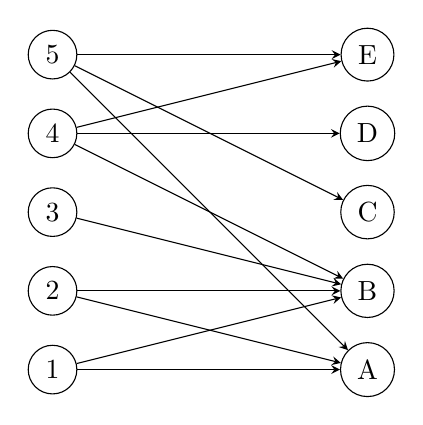
\begin{tikzpicture}
        \node[draw,circle] (1) at (0,1){1};
        \node[draw,circle] (2) at (0,2){2};
        \node[draw,circle] (3) at (0,3){3};
        \node[draw,circle] (4) at (0,4){4};
        \node[draw,circle] (5) at (0,5){5};
        \node[draw,circle] (A) at (4,1){A};
        \node[draw,circle] (B) at (4,2){B};
        \node[draw,circle] (C) at (4,3){C};
        \node[draw,circle] (D) at (4,4){D};
        \node[draw,circle] (E) at (4,5){E};

        \path [draw,->,>=stealth] (1) to (A);
        \path [draw,->,>=stealth] (1) to (B);
        \path [draw,->,>=stealth] (2) to (A);
        \path [draw,->,>=stealth] (2) to (B);
        \path [draw,->,>=stealth] (3) to (B);
        \path [draw,->,>=stealth] (4) to (B);
        \path [draw,->,>=stealth] (4) to (D);
        \path [draw,->,>=stealth] (4) to (E);
        \path [draw,->,>=stealth] (5) to (A);
        \path [draw,->,>=stealth] (5) to (C);
        \path [draw,->,>=stealth] (5) to (E);
    \end{tikzpicture}
    \caption{Une flèche de $i$ vers $j$ représente que $j$ sait utiliser le scanner $i$.}
    \label{fig:scan}
\end{figure}

\begin{parts}
    \part En supposant que les 5 employés sont disponibles. Combien de scans peuvent être effectués en même temps ?
\begin{solutionbox}{4.5cm}
    Les scanners 1, 2, 3 ne peuvent qu'être utilisés par A et B donc on ne sait pas utiliser ces 3 scanners en même temps.
    On ne sait donc utiliser que 4 scanners à la fois.
\end{solutionbox}
    \part Proposer une formation à l'utilisation d'un scan pour un employé qui augmenterait le nombre de scans pouvant être effectués simultanément.
\begin{solutionbox}{4.5cm}
    Il faut former C, D ou E à l'utilisation d'un des scanners 1, 2 ou 3.
\end{solutionbox}

Suite à l'apparition d'une pandémie, l'état à investit massivement dans l’hôpital.
Il y a maintenant 100 scanners et 100 employés pouvant effectuer les scans.

    \part Quel algorithme pouvez-vous utiliser pour résoudre ce problème efficacement ? (\emph{Indice: il faut peut-être ajouter des nœuds fictifs au graphe de la Figure~\ref{fig:scan} pour que ça corresponde à un des problèmes vu en cours...})
    \part Comment trouver quelle formation proposer pour augmenter la capacité de scan de l’hôpital à partir de la solution du problème ?
\begin{solutionbox}{17cm}
    On ajoute une source qui relie à tous les scanner et on relie tous les employés à une source.
    Ça donne une problème de Max-Flow avec une capacité de 1 pour toutes les arêtes:
    De façon équivalente, le Max-Flow est égal à Min-Cut. La solution du Min-Cut est de groupé les nœuds
    bleus et verts comme ci-dessous.
    La coupe est alors formée par les arêtes en rouges qui relient un nœud bleu
    à un nœud vert.

    Il faut former un employé dont la solution du Max-Flow donne une valeur de 0
    à son arête vers T à utiliser un scanner dont la solution du Max-Flow donne
    une valeur de 0 à l'arête le reliant à S.
    \begin{center}
    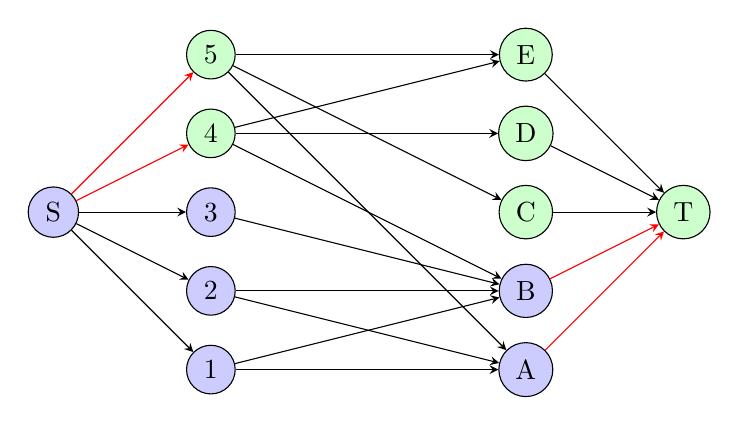
\begin{tikzpicture}
        \node[draw,circle,fill=blue!20] (1) at (0,1){1};
        \node[draw,circle,fill=blue!20] (2) at (0,2){2};
        \node[draw,circle,fill=blue!20] (3) at (0,3){3};
        \node[draw,circle,fill=green!20] (4) at (0,4){4};
        \node[draw,circle,fill=green!20] (5) at (0,5){5};
        \node[draw,circle,fill=blue!20] (A) at (4,1){A};
        \node[draw,circle,fill=blue!20] (B) at (4,2){B};
        \node[draw,circle,fill=green!20] (C) at (4,3){C};
        \node[draw,circle,fill=green!20] (D) at (4,4){D};
        \node[draw,circle,fill=green!20] (E) at (4,5){E};

        \path [draw,->,>=stealth] (1) to (A);
        \path [draw,->,>=stealth] (1) to (B);
        \path [draw,->,>=stealth] (2) to (A);
        \path [draw,->,>=stealth] (2) to (B);
        \path [draw,->,>=stealth] (3) to (B);
        \path [draw,->,>=stealth] (4) to (B);
        \path [draw,->,>=stealth] (4) to (D);
        \path [draw,->,>=stealth] (4) to (E);
        \path [draw,->,>=stealth] (5) to (A);
        \path [draw,->,>=stealth] (5) to (C);
        \path [draw,->,>=stealth] (5) to (E);
        \node[draw,circle,fill=blue!20] (S) at (-2,3){S};
        \node[draw,circle,fill=green!20] (T) at (6,3){T};
        \path [draw,->,>=stealth] (S) to (1);
        \path [draw,->,>=stealth] (S) to (2);
        \path [draw,->,>=stealth] (S) to (3);
        \path [draw,->,>=stealth,color=red] (S) to (4);
        \path [draw,->,>=stealth,color=red] (S) to (5);
        \path [draw,->,>=stealth,color=red] (A) to (T);
        \path [draw,->,>=stealth,color=red] (B) to (T);
        \path [draw,->,>=stealth] (C) to (T);
        \path [draw,->,>=stealth] (D) to (T);
        \path [draw,->,>=stealth] (E) to (T);
    \end{tikzpicture}
\end{center}

\end{solutionbox}
\end{parts}
